\documentclass[a4paper,12pt]{scrartcl}

\usepackage[utf8]{inputenc}
\usepackage[ngerman]{babel}
\usepackage[T1]{fontenc}
\usepackage{graphicx}
\usepackage{lmodern}
\usepackage{tabto}
\usepackage{listings}
\usepackage[backend=biber, style=authoryear]{biblatex}
\addbibresource{referenzen.bib}



\title{Implementierung von Kryptologie in Programmiersprachen}
\subtitle{Kryptologie 2}
\author{Moritz Rupp}
\date{Wintersemester 2020}


% Mathepakete
\usepackage{amsfonts}
\usepackage{amsmath}


\begin{document}

\maketitle
\newpage
\tableofcontents
\newpage


\section{Abstract}

Die vorliegende Arbeit gibt einen Überblick auf verschiedenste Implementierungen von Kryptografie in Programmiersprachen. Dabei werden Kriterien wie die Schutzziele der Informationssicherheit in Form von Vertraulichkeit, Integrität und Verfügbarkeit auf ausgewählte Sprachen angewand und vergleichen. Da Software Biblotheken die direkteste Umsetzung von Kryptologie in Programmiersprachen darstellen werden auf diese ein Hauptaugenmerk gelegt! Des weiteren ist es Ziel die Stärken und Schwächen der jeweiligen Programmiersprachen auszumachen und dementsprchend ihrem idealen Anwendungsbereich in der Kryptografie zuzuordnen! Da nahezu alle modernen High-Level Sprachen auf sogenannten Low-Level bzw. Speichernahen Sprachen wie Assemply und C aufgebaut sind, werden diese anfangs unter die Lupe genommen um anschließend 'High Level' Sprachen wie C++, Java und Python zu untersuchen. Zur Veranschaulichung werden ausgewählte Krypto-Algorithmen nachprogrammiert, was nicht der allgemeinen Empfehlung entspricht.
Eines der wichtigsten Regeln der Kryptografie besagt nähmlich man solle nie seine eigene Krypto schreiben.
Das heißt dass man die Verschlüsselungsalgorithmen niemals selbst programmieren oder gar neue, für sich maßgeschneiderte Implementierungen erstellen sollte. Ein Grund dafür ist die extrem hohe Anfälligkeit die solche Versuche mit sich führen würden.
Etablierte Kryptografische Verfahren haben einen langen Testprozess durchlaufen. Über viele Jahre werden sie von Experten der Prüfung unterzogen. Trotzdem gibt es immer wieder erfolgreiche Angriffe auf vermeintlich sichere Krypto. Der Schwachpunkt liegt hierbei häufig nicht in dem Kryptografischen Verfahren an sich, sondern an der falschen Implementierung der Software Anwendung! Deshalb sollten bei Anwendung von Kryptografie in Software nicht nur Aspekte wie Schnelligkeit und Effizients eine Rolle spielen, sondern die Anforderungen um Sicherheit auch bei voller Transparanz des Codes erweitert werden. Kerkocks Prinzip sollte also auch übertragen auf Software Implementierungen von Kryptografie gelten! Dieser Grundsatz beschreibt das die Sicherheit eines Verschlüsselungsverfahren allein durch Geheimhaltung des Schlüssels sicher gestellt wird, nicht aber durch Geheimhaltung des Verschlüsselungsalgorythmus! Auf Software bezogen heißt dieß, das selbst bei Veröffentlichung des Quellcodes die Kryptografische Sicherheit der Anwendung bestehen sollte. Kontrolliert umgesetzt wird dies in Form von Open-Source Projekten! 
Es zeigt sich das diese eine höhere Sicherheit aufweisen als closed-source Projekte! Ein Grund dafür ist Tatsache das dass Code Design von Grund auf entsprechend ausgelegt wird! Werden closed-source Projekte komprementiert und somit der Quell-Code veröffentlicht, stellt man oft fest das die Sicherheit hierbei nicht im Code selber liegt. Durch die Einsicht des Quellcodes von deutlich mehr Entwicklern als bei closed-source werden zudem speziell in Verbindung mit Entwicklungsplattformen wie GitHub/Gitlab deutlich mehr Sicherheitslücken und generelle Bugs aufgedeckt.
Häufige Fehlerquellen bei Krypto-Implementierungen sind schlechte pseudo Zufallszahlengeneratoren, falsche bzw. unsichere Betriebsmodi wie zB. ECB, oder das Verwenden von gleichbleibenden, symetrischen Schlüsseln! \newpage
Die vorgestellten Programmiersprachen sind unterschiedlich anfallig für solche Schwachstellen und werden dementsprchend Bewertet bzw. ihrem idealen Anwendungsbereich zugeordnet!\footnote{Buchmann2016}



 
\newpage


\section{Assembly}
Assemblysprachen stellen die tiefste Ebene der Programmiersprachen dar.
Sie laufen extrem Hardware nah und können dadurch alle Möglichkeiten eines Mikroprozessors nutzen. Dies ist zwar heutzutage meist nicht erforderlich, kann aber auf kleineren Endgeräten wie Iot devices durchaus nützlich sein, weshalb gewisse Anwendungen immer noch in 'plain' Assembly code geschrieben werden.\\ Durch die Hardware nähe und die daraus resultierende Schnelligkeit könnte man denken das sich Assembly Code gut für Kryptografie eignet. Der Aufwand und die Komplexität ein Krypto Algorythmus in Assembly zu realisieren sind jedoch meist zu groß sodass 'High level' Sprachen beforzugt werden.\\
Ein weiterer Nachteil ist die Tatsache das Assembleysprachen sehr spezialisiert auf die jeweiligen Computerarchitekturen ausgelegt sind. Das heißt das Spezifikationen und Befehlssätze nur auf dieser bestimmten Auslegung laufen. Dies hat zur Folge das die Übertragung auf eine andere Architektur mit sehr viel Aufwand und Anpassung im Quelltext verbunden wäre!\\
Des weiteren haben die wenigsten Assembleysprachen die Notwendigen Operationen bzw. Befehle die für Kryptografisches arbeiten Notwendig sind. Einfache arithmetische Operationen wie Addition oder Vergleiche von Ganzzahlen sind zwar vorhanden, komplexere Operationen wie Modulo Rechung oder Gleitkommaarithmetik nur vereinzelt und müssten sonst von Grund auf eigens definiert werden!\\
Trotz der vielen genannten Nachteile gibt es Verwendung in Bereichen in denen 'High level' Sprachen nicht genug Effizients bieten. Implementierungen in C sind zwar wesentlich einfacher zu schreiben und lesen, jedoch wäre eine Optimierte Umsetzung des gleichen Programmes in Assembly trotz moderner hoch optimierter Compiler für gewisse Aufgaben schneller.\\
Der vom C Compiler generierte Assembly code ist also potenziell schlechter bzw. ineffizienter als ein von Menschen geschriebener Assembly code!\\ Ein Grund dafür ist die Tatsache das Compiler schlecht mit großen Zahlen umgehen können. Das heißt speziell in Kryptografie in der viel und oft mit großen Integers gearbeitet wird ist es durchaus sinnvoll gewisse Rechenoperation in 'plain Assembly code' zu realisieren.\footnote{\cite{738514}}
\newpage
Folgendes Beispiel veranschaulicht dies indem ein einfaches Programm in C anhand von GCC kompiliert wird. Anschließend wird die gleiche Operation in 'plain Assembly' nachgeschrieben. Wie sich zeigt ist der von GCC generierte Assemblycode wesentlich länger und langsamer.\\
Das C Programm realisiert das Modul addcarry u64, welches die Summe zweier 'unsigned Integer' und einem carry-in computiert und den Wert des carrys outs zurückgibt!
\vspace{2 mm}

\begin{lstlisting}
#include <stdint.h>
#include <x86intrin.h>

void add256(uint64_t a[4], uint64_t b[4]){
	uint8_t carry = 0;
	for (int i = 0; i < 4; ++i)
		carry = _addcarry_u64(carry, a[i], b[i], &a[i]);
}
\end{lstlisting}
\vspace{7 mm}
Nun der von GCC kompilierte Assemblycode:
\begin{lstlisting}
add256:
movq    (%rsi), %rax
addq    (%rdi), %rax
setc    %dl
movq    %rax, (%rdi)
movq    8(%rdi), %rax
addb    $-1, %dl
adcq    8(%rsi), %rax
setc    %dl
movq    %rax, 8(%rdi)
movq    16(%rdi), %rax
addb    $-1, %dl
adcq    16(%rsi), %rax
setc    %dl
movq    %rax, 16(%rdi)
movq    24(%rsi), %rax
addb    $-1, %dl
adcq    %rax, 24(%rdi)
ret
\end{lstlisting}
\newpage
Schreibt man das Programm nun in optimiertem Assemblycode zeigt sich das dieser wensentlich kompakter ist! \\


\begin{lstlisting}
add256:
movq    (%rsi), %rax
addq    %rax, (%rdi)
movq    8(%rsi), %rax
adcq    %rax, 8(%rdi)
movq    16(%rsi), %rax
adcq    %rax, 16(%rdi)
movq    24(%rsi), %rax
adcq    %rax, 24(%rdi)
retq
\end{lstlisting}
Auch Laufzeiten sind merklich verkürzt!
Je nach Kompiler und Architektur kann selbst geschriebener Assemblycode bis zu doppelt so schnell wie kompilierter Code sein!
\\
Stellen wir also fest das 'plain' Assemblycode durch seine schnelligkeit und Effizients für gewisse Aufgaben und spezialisierte Bereiche durchaus einen Vorteil gegenüber High level Sprachen bietet!\\
Die Frage ist nun ob das auch für Kryptografische Anwendungen gilt?!\\
Wie anfangs erwähnt sind in den meisten Assembly Sprachen nicht alle notwendigen Operationen wie modulo Rechnung vorhanden. So könnte man diese zwar eigens nachprogrammieren, jedoch stünde der Aufwand in keinem Verhältnis zu der schnelleren Laufzeit die man dadurch gewinnen würde.\\
Das hat zur Folge das in praxis kaum komplexere Krypto Anwendungen in 'plain' Assembly geschrieben werden! Stattdessen werden kleine Verschlüsselungsalgorythmen wie TEA oder Rot13 realisiert.\footnote{Vorlesungsfolien}\\
Im folgenden wird der Tiny Encryption Algorithm in Assembly implementiert. Dieser ist eine Blockverschlüsselung die für Ihre einfachheit, Kompaktheit und daraus resultierende Schnelligkeit bekannt ist. 
TEA ist eine Feistelchiffre und arbeitet mit 64-Bit Blöcken und einem 127-bit langem Schlüssel.\\
Der Assemblycode ist in der x86 Architektur geschrieben.\footnote{\cite{738514}}









\newpage
\textbf{Tiny Encryption Algorythm on Assembly x86}
\begin{lstlisting}
pushl  %ebp
movl   %esp, %ebp 	Eingabe 3 Woerter und Zweisung Lokalem Speicher 
subl   $12, %esp	auf den Stack

movl   %ebx, 0(%esp)
movl   %esi, 4(%esp)	Speichern der callee-save registers
movl   %edi, 8(%esp)

movl    8(%ebp), %eax  
movl   12(%ebp), %edx  	Einladen des Message arrays!

movl   0(%eax), %esi	Einladen beider 32-bit Woerter
movl   4(%eax), %edi	der Nachricht
movl   $0x9E3779B9, %ecx 

.tea_encrypt_top:	Beginn der Schleife

movl   %edi, %ebx
shll   $4, %ebx
addl   0(%edx), %ebx
leal   (%edi,%ecx), %eax
xorl   %eax, %ebx
movl   %edi, %eax	Verschluesselung der Nullten Nachricht.
shrl   $5, %eax
addl   4(%edx), %eax
xorl   %eax, %ebx
addl   %ebx, %esi

movl   %esi, %ebx
shll   $4, %ebx
addl   8(%edx), %ebx
leal   (%esi,%ecx), %eax
xorl   %eax, %ebx	Verschluesselung der ersten Nachricht
movl   %esi, %eax	ueber den selben Weg
shrl   $5, %eax
addl   12(%edx), %eax
xorl   %eax, %ebx
addl   %ebx, %edi
 
 addl   $0x9E3779B9, %ecx
 cmpl   $0x6526B0D9, %ecx  Erhoehung der Runden Konstanten.
 jne    .tea_encrypt_top
 
 movl   8(%ebp), %eax
 movl   %esi, 0(%eax)	Ende der Schleife. Speicherung der Nachricht
 movl   %edi, 4(%eax)	in einem Array
 
 movl   0(%esp), %ebx
 movl   4(%esp), %esi	
 movl   8(%esp), %edi
 
 addl   $12, %esp	Freigeben des Stacks 
 popl   %ebp	
 retl
\end{lstlisting}
\vspace{10mm}
Ein Vorteil der x86 Architektur ist die Tatsache das arithmetische operationen aus dem Speicher lesen und schreiben können. Daraus resultiert die relative kompaktheit des codes! Dies ist jedoch nicht für alle Assembly Sprachen gegeben!\footnote{\cite{738514}}
\subsection{Sicherheit}
Assemblycode an sich verfügt über nahezu keine eingabauten Sicherheitsstrukturen. Datenkapselung bzw. Objektorientierung sind zwar theoretisch nachbildbar, jedoch praktisch kaum anwendbar! Denoch spielen Assembleysprachen eine wichtige Rolle in der It-Security! Durch die Hardware nähe ist es möglich Code auf Bitebene zu verändern. Dies ist zwar auch mit gewissen High-level sprachen möglich, jedoch nicht ansatzweise so nachvollziebar!\footnote{Vorlesungsfolien}\\
Assemblycode wird beispielweise oft verwendet um Speicherüberläufe zu entwickeln bzw. auszunutzen.
\subsection{Biblotheken}
Von Biblotheken in 'plain' Assembly kann man nicht wirklich Sprechen. Vielmehr existieren Biblotheken in  C/C++ die man je nach Architektur auch für Assembly verwenden kann.
Dadurch  das es nicht eine bestimmte Assemblysprache gibt, existiert beispielweise auch keine Standart Biblothek. Jede Architektur hat ihre eigenen module und Implementierungen. Durch diese fehlende Einheitlichkeit gibt es wenig Dokumentation speziell im Bereich Kryptologie!\\
Denoch existieren beispielweise  in ssl oder Libsodium Implementierungen in 'Hand geschriebenem' Assembly!


\newpage
\section{C}
C ist eine alte, aber dennoch sehr verbreitete und genutze Sprache. \\Heutzutage wird sie als extrem Hardware-nah bezeichnet, ist im gegensatz zu Assembly jedoch durchaus als 'High level' Sprache zu bezeichnen. Ein riesen Vorteil gegenüber Assembleysprachen ist die viel bessere lesbarkeit und Plattformunabhängigkeit.
Auch sind nahezu alle Mathematischen Operationen die für Krypto-Anwendungen benötigt werden vorhanden oder können einfach durch diverse Biblotheken eingebunden werden. Des weiteren ist C im Vergleich zu heutigen 'High level' Sprachen extrem schnell. Zwar gibt es wie erwähnt gewisse Fälle in denen Kompiler Optimierungsprobleme haben, jedoch gilt dies nur im direkten Vergleich zu Assembly Sprachen!\footnote{https://bhavikjoshi35.wordpress.com/2015/12/10/c-programming-language/}\\
\subsection{Sicherheit}
Nachteile der Sprache sind, insbesondere bezogen auf Kryptografie die hohe Anzahl an sicherheitsrelevanten Fehlermöglichkeiten. Dadurch das ein Programmierer nahezu uneingeschränkt mit Zeigern und Speicherstrukturen arbeiten kann und Kompiler nur teilweise auf Sicherheit prüfen gibt es ein recht hohes Potential Angreifbare Fehler zu produzieren.
Unter anderem sind das:
\begin{itemize}
 \item Hängende Zeiger\\
 Zeiger die auf gar keinen oder den falschen Speicherbereich verweisen. Dies kann bei Implementierung eines Krypto-Algorythmus in C zu unsicherheiten oder dem kompletten Ausfall der Anwendung führen!
  
 \item Pufferüberlauf\\
  Ein zu klein verwiesener Speicher kann dazu führen das auch hier schadcode Platziert werden kann oder das Programm abstürzt!
  \item Race conditions\\
  Dieser Fehler tritt auf wenn zeitliche koordinierung von Programmaufgaben schlecht oder gar nicht Synchroniziert werden. Klassische Beispiele sind Signale in der Systemprogrammierung oder Speicher operationen auf einem Mikroprozessor.
  
 
\end{itemize}
Des weiteren exisiert keine automatische Laufzeitüberpürfung, was beispielweise bei Kryptoanalysen Probleme bereitet.\\
Die Eignung von C für Krypto-Anwendungen hängt also stark von der Expertise des Programmierers ab! Ist dieser in der Lage die erwähnten Risiken zu entschärfen bzw. zu umgehen, überwiegen die erwähnten Vorteile von Schnelligkeit und Effizients!\newpage
In Realität gibt es jedoch immer wieder Fälle bei denen schlechter, unsicherer C Code zu gefährlichen Sicherheitslücken führt! Schaut man sich beispielweise die Patch notes von Mozilla Firefox an, fällt auf das viele Schwachstellen auf genau solch Probleme zurückzuführen sind! Monatlich gibt es bis zu 10 mittlere, teilweise schwerwiegende Sicherheitsfixes, die meist durch Speicherüberläufe in C/C++ entstehen.\footnote{Vorlesungsfolien}
\newpage
Ein berühmter sehr kostspieliger Fall trat 2014 in Form des 'Heartbleed' exploites auf. Diese Lücke machte es Angreifern möglich sensitive Informationen wie Passwörter oder Bankdaten von Webseiten abzugreifen. Zurückzuführen war das ganze auf eine Fehlerhafte Speicherimplementierung in OpenSSl was in C geschrieben ist. 
OpenSSl ist eine Software-Biblothek die verschiedene Netzwerkprotokolle und Verschlüsselungen umfasst, unter anderem TLS bzw. SSL. Diese werden genutzt um eine sichere Datenübertragung  zwischen Client und Host zu gewährleisten. Grob beschrieben führt TLS ein Handshake durch, bei dem ein Schlüsselaustauch sowie eine Authentisierung stattfindet. Über den TLS Record wird nun anhand des Schlüssels eine sichere Verbindung aufgebaut. Um zu gewährleisten das diese sichere Verbidung auch nach längerer inaktivität gegeben ist, sendet TLS regelmäßig einen sogenannten 'heartbeat request'. Dieser besteht aus einem chiffrierten Datenblock. Der Empfänger antwortet mit dem exakt gleiche Datenstück und beweist damit das die sichere Verbindung noch besteht! Wichtig hierbei ist das die ursprüngliche Anfrage Informationen über seine länge enthählt. Dadurch weiß der Empfänger wie viel Speicher für die Nachricht freigeben muss. An diesem Punkt trat die Schwachstelle auf. Seitens des Empfängers wurde nähmlich nicht überprüft ob die angegebene lönge stimmte! Das heißt ein 'heartbeat request' konnte mit 50kb angegeben sein, hatte jedoch eine tatsächliche länge von nur 25kb. Der betrofene Empfänger gab also diese 50kb frei, speicherte die eigentlichen 25kb und versand diese anschließend wieder mitsamt 25kb weiterer Daten die sich in diesem Speicher befanden! Der Angreifer hat nun also diese Daten seitens des Empfängers abgegriffen. Dies zeigt wie schnell unsauberer Code in katastrophalen Schwachstellen enden kann. Der Auslöser des ganzen kann auf eine einzelne Zeile im C Code zurückgeführt werden:

\begin{center}
\begin{lstlisting}
	{
		memcpy(bp, pl, payload);
	}
\end{lstlisting}
Das Kommando 'memcpy()' kopiert Daten aus dem Speicher 'pl' in 'pb'.\\ Das Argument 'payload' gibt die länge des kopierten Datenstückes an!\\ 
\end{center}
Trotz der Tatsache das OpenSSl damals wie heute Open Source ist und somit jeder diese Sicherheitslücke hätte sehen können, wurde dies erst in Folge des heartbleed exploites gefixt! Dies zeigt erneut das Risiko Krypto Anwendungen in C zu schreiben!\\
Denoch ist C die wahrscheinlich meist genutzte Sprache um Kryptografische Anwendungen umzusetzen. Auch viele Verschlüsselungsbiblotheken von anderen Sprachen, sind letztendlich C Verbunde!\footnote{https://blog.malwarebytes.com/exploits-and-vulnerabilities/2019/09/everything-you-need-to-know-about-the-heartbleed-vulnerability/}
\vspace{2.5mm}
\newpage
Obwohl Biblotheken viele arbeiten wie Hashing/Chiffrierung etc. abnehmen, kann man diese Operationen natürlich auch selber in 'plain' C nachschreiben. Dies wird im folgenden anhand des One time Pads gezeigt! 




\begin{verbatim}
#include<stdio.h>
#include<string.h>
#include<ctype.h>

main(int argc, char *argv[])
{
    //Jegliche Eingaben werden in Großbuchstaben convertiert 
    //und Leerzeilen werden entfernt.
    int i,j,len1,len2,numstr[100],numkey[100],numcipher[100];
    char str[100],key[100],cipher[100];
    printf("Bitte geben Sie den zu verschlüsselnden Text ein\n");
    gets(str);
    for(i=0,j=0;i<strlen(str);i++) {
        if(str[i]!=' ') {
             str[j]=toupper(str[i]);   //toupper ist eine C interne Funktion
             j++;                      //die hier anhand einer For-Schleife
        }                              //die Eingaben in Großbuchstaben umschreibt
    }
    str[j]='\0';
    //Erhalt des Klartextes (nummerisch)
    for(i=0;i<strlen(str);i++) {
       numstr[i]=str[i]-'A';    
    }   
    printf("Bitte einen Zufälligen Text eingeben(Länge beliebig)\n");
    gets(key);
    for(i=0,j=0;i<strlen(key);i++) {
        if(key[i]!=' ') {
            key[j]=toupper(key[i]);   
            j++;
        }
    }
    key[j]='\0';
    //Erhalt des OTP bzw. Key
    for(i=0;i<strlen(key);i++) {
        numkey[i]=key[i]-'A';    
    }  

    for(i=0;i<strlen(str);i++) {
        numcipher[i]=numstr[i]+numkey[i];
    }
   
    for(i=0;i<strlen(str);i++) {
        if(numcipher[i]>25) {
           numcipher[i]=numcipher[i]-26;
        }
    }
    printf("Der One Time Pad Ciphertext ist\n");
    for(i=0;i<strlen(str);i++) {
        printf("%c",(numcipher[i]+'A')); 
    }
    printf("\n");

}

\end{verbatim}

Durch benutzen von 'gets()' setzt man das Programm ein recht hohes Risiko zu einem Buffer Overflow aus! Deshalb gilt die ungeschriebene Regel ' Dont write your own krypto'.\footnote{https://www.educba.com/one-time-pad/}
Bei Ausführung des Programmes zeigt sich folgendes:
\begin{figure}[h]

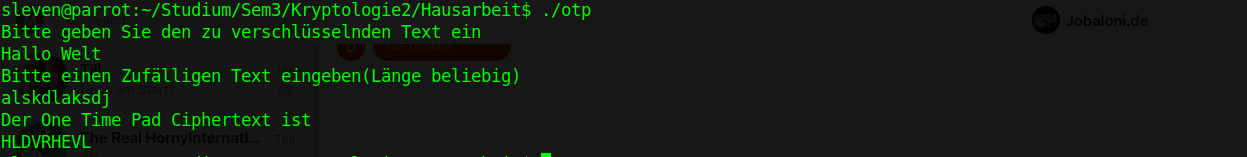
\includegraphics[scale=0.41]{otp.png}     
\end{figure}


\newpage
\subsection{Biblotheken}
Als C 1976 erschien, war die Notwendigkeit von kryptographischen Verfahren und deren Implementierung noch lange nicht so hoch wie heute. Daher gab es anfangs auch wenige Bibliotheken speziell im Krypto-Bereich! Inzwischen hat C jedoch  eine breite Auswahl an Bibliotheken für kryptographische Verfahren die heute noch regelmäßig Updates bekommen.\\

\vspace{2mm}
\textbf{OpenSSL}: Die wohl bekannteste und meist genutzte Biblothek für Kryptografie. Nahezu alle HTTPS Websites nutzen diese Biblothek.\\

Um OpenSSL für C Code zu verwenden sollten folgende Header eingebunden werden.
\begin{verbatim}
#include <openssl/evp.h>
#include <openssl/ssl.h>
#include <openssl/rsa.h>
#include <openssl/x509.h>
\end{verbatim}
Je nach Verwendung müssen nun die notwendigen Initialisierungen durchgeführt werden. Dies könnte man anhand folgender Funktion umsetzen:
\begin{verbatim}
void init_ssl() {
     SSL_library_init(); 
     SSL_load_error_strings();
     ....
}
\end{verbatim}
Folgender Funktionsauschnitt generiert beispielweise einen RSA Key:
\begin{verbatim}
RSA *rsa;
rsa = RSA_new();
//RSA_generate_key_ex(r, bits, bn, NULL);

RSA_generate_key_ex(
	r,  // Zeiger auf RSA Struktur 
	bits, // Anzahl der bits für den Schlüssel zB. 2048
	bn,   // Zugeteilter Exponent  
	NULL, // Callback 
);

\end{verbatim}
Hier wird anschaulich lediglich ein einzelner Key generiert! Ein vollständiges Programm müsste zudem den Public und Private Key noch zwischenspeichern.\footnote{Vorlesungsfolien}

\newpage
Auch ist es möglich OpenSSl Kommandos die eigentlich in einer Shell ausgeführt werden in C Code zu implementieren.
Folgendes Kommando Generiert einen Private Key und ein Zertifikat.\\

\textbf{openssl req -out geekflare.csr -newkey rsa:2048 -nodes -keyout geekflare.key}

In einem C Programm eingebunden:
\begin{verbatim}
int main () {
   char c[50]; 
   strcpy( c, "openssl req -out geekflate.csr -newkey rsa:2084 ...." );
   system(c);
   return 0;
} 
\end{verbatim}
Diese Umsetzung von OpenSSL in C ist jedoch nur für kleinere Anwendungen\\ gebräuchlich!\\
\\
\textbf{Cryptlib}:
Bietet ein High-Level Interface zur einfachen Implementierung von Sicherheits-
funktionen. Sie ist komplett in C geschrieben, kann und wird aber auch in JAVA, C++ und weiteren Sprachen verwendet. Cryptlib umfasst unter anderem SSL/TLS, OpenPGP, MIME und viele weitere Protokolle und Standarts. Auch Krypto-Algorithmen wie AES,DES, RSA oder SHA-1/2 sind vertreten. Für die Verwendung in C Code sind 
folgende Header zu verwenden:\footnote{\cite{1028896}}
\begin{verbatim}
#include "cryptlib.h"
\end{verbatim}
Initialisierungen:
\begin{verbatim}
using cryptlib;
crypt.Init();
...
crypt.End();
\end{verbatim}
Hier wird nun eine Anwendung mit Sha realisiert:
\begin{verbatim}
Encrypt:
var cryptLib = require(’cryptlib’),
iv = cryptLib.generateRandomIV(16), //16 bytes = 128 bit
key = cryptLib.getHashSha256(’my secret key’, 32), //32 bytes = 256 bits
encryptedText = cryptLib.encrypt(’This is the text to be encrypted’, key, iv);
Decrypt:
var cryptLib = require(’cryptlib’),
iv = ’iv vector used for encryption’,
key = cryptLib.getHashSha256(’my secret key’, 32), //32 bytes = 256 bits
originalText = cryptLib.decrypt(’M2rfrn9DqNHJe3Hev9nMxKKgIHoqUsc7FJM+tBGxIrl3Wk9UeKIQ
\end{verbatim}
\dots
\newpage
Weitere Relevante Krypto Biblotheken sind:
\begin{itemize}
\item libsodium \\Bietet Verschlüsselung, Entschlüsselung, Signaturen, Passwort-Hashing und mehr. Sie ist plattform- und sprachenübergreifend und läuft auf einer Vielzahl von Compilern und Betriebssystemen, einschließlich Windows.

\item LibreSSL\\
Ist eine open-source implementierung des TLS Protokolls. Es läuft auf  	OpenBSD, FreeBSD, Solaris, Linux, macOS und Windows.
\item Libgcrypt\\
Basiert auf GnuPG und bietet eine breite Anzahl allgemeiner Symetrischer Verschlüsselungs Algorythmen wie AES, DES, ChaCha20 mitsamt einer vielzahl von Betriebsmodi. 
\item wolfCrypt\\
Eine open-source SSL Programmbiblothek die speziell für Entwickler von Embedded-Systemen geeignet ist.

\end{itemize}

Es existieren mehr als 20 aktiv geführte Krypto Biblotheken in C. Dazu kommen etliche Github Repos die Krypto Anwendungen realisieren.\\
Nimmt man dies alles zusammen stellt man fest das C nach wie vor die universellste und meist genutze Sprache für Krypotgrafie ist!\footnote{\cite{1028896}}

\newpage
\section{C++}
C++ ist sehr nah an C aufgebaut und kann als direkter Nachfolger der Sprache bezeichnet werden. Aus heutiger Sicht, bzw. im Vergleich zu modernen Sprachen ist  auch sie als 'Low level' Programmiersprache einzuordnen. Funktionen wie freie Speicherverwaltung seitens des Programmierers oder arbeiten mit Zeigern sind vorhanden und teilweise ähnlich wie in C implementiert. Grundsätzlich weisen die beiden Sprachen eine recht hohe Ähnlichkeit auf, die sich jedoch größtenteils in Form der Notation bzw. Syntax äußert! Weitere Gemeinsamkeiten sind die allgemeine Code Struktur sowie Schlüsselwörter und Operatoren. Auch das Speichermodell ist orientiert an C, sehr nahe an der Hardware aufgebaut.\\
Denoch bestehen grundlegende Unterschiede zwischen beiden Sprachen!\\
So ist in C++ Objektorientierte Programmierung möglich. Dies lässt sich zwar in C anhand von 'structs' nachmodellieren, jedoch ist durch die Einführung der Klasse in C++ ein deutlich höheres Abstractionsniveau möglich!\\
Würde man in C beispielweise eine Matrix implementieren, so müsste man mehrer arrays anlegen und zwischen diesen Relationen herstellen. In C++ lässt sich dies wesentlich einfacher in Form der Klasse Matrix umsetzen.\\
Weitere Vorteile stellen Funktionen wie Excpeption Handling(Ausnahmebehandlung) oder Vererbung dar. Diese sind insbesondere auch für die Erstellung  Krypotgrafischer Anwendungen von Vorteil.\footnote{\cite{HAMMI2018126}}

\subsection{Sicherheit}
Durch die Nähe zu C gelten nahezu alle Sichersrelevanten Schwachstellen auch in C++. Hängende Zeiger und Buffer Overflows sind genauso ein Problem wie Race conditions. Dennoch bietet C++ durch die Objektorientierung mehr Sicherheit. So können Variablen besser versteckt bzw. geschütz werden durch Abkapselung in Klassen!\\
Festhalten kann man das C++ durch einige Verbesserungen der Code Sicherheit durchaus eine bessere Eignung für Krypo-Anwendungen aufweißt. Dies zeigt sich auch in der Anzahl der realisierten Konzepte in diesem Bereich!\\
Viele bekannte Blockchain Projekte wie Bitcoin, Ethereum und Ripple sind in C++ verfasst.\footnote{Vorlesungsfolien}
\newpage
\subsection{Bibliotheken}
Auch C++ wurde bei Veröffentlichung 1985 nicht unbedingt für Kryptografische Zwecke entwickelt. Die Standart Biblothek enthält zwar mehr als in C, Funktionen die für Kryptografische Zwecke nützlich sind, denoch ist man bei größeren Krypto-Anwendungen auf neuere externe Biblotheken angewiesen! Davon gibt es heutzutage allerdings eine Vielzahl!\\
Hinzu kommt das nahezu alle C Biblotheken bzw. Header auch in C++ verwendbar sind. Diese müssen jedoch speziell deklariert werden!\\ 
Möchte man beispielweise aus C eine Standartbiblothek in C++ verwenden, muss man lediglich die '.h' Endung entfernen und ein 'c' prefix hinzufügen.\\ So wird aus: \begin{verbatim}
#include <stdio.h>       #include <cstdio>
\end{verbatim}
Will man andere Header verwenden die nicht teil der Standartbiblothek sind so geht das wie folgt:
\begin{verbatim}
extern "C"
{
    #include "weitere_header.h"
}                                                                                          \end{verbatim}
Viele C Biblotheken werden inzwischen durch C++ ergänzt bzw. weitergeführt. So ist \textbf{OpenSSL} in beiden Sprachen verwendbar und gebräuchlich!\\
Für \textbf{cryptlib} gilt das gleiche!\\
\vspace{1mm}\\
\textbf{Crypto++}:\\ Erstmals Veröffentlicht 1995 von Wei Dai. Seit 2015 arbeitet the Crypto++ Project daran weiter.\\
\vspace{1mm}\\
\textbf{Libtomcrypt}:\\
Bietet ähnliche Protokolle und Algorithmen wie OpenSLL. Jedoch deutlich einfacher gehalten. Wird auch als 'lighweight openssl' bezeichnet!\\Libtomcrypt besitz eine Public Domain licence!\footnote{\cite{HAMMI2018126}}
\newpage
\textbf{Botan}:\\ 
Die wahrscheinlich wichtigste und Größte Krypto-Biblothek in C++!\\ Vom BSI evaluiert und für den Einsatz in Sicherheitsprodukten geeignet, klassifiziert. Bis heute regelmäßig durch das BSI geprüft.\\

Zu Beginn wird ein LibraryInitializer-Objekt erstellt. Mit diesem werden verschieden in
terne Strukturen auf und abgebaut.
\begin{verbatim}
 #include <botan/botan.h>
int main()
{
	LibraryInitializer init;
	return 0;
}
S2K* s2k = get_s2k("PBKDF2(SHA-256)");
s2k->set_iterations(4096);
s2k->new_random_salt(8);
SecureVector<byte> the_salt = s2k->current_salt();
SymmetricKey master_key = s2k->derive_key(48, passphrase);
KDF* kdf = get_kdf("KDF2(SHA-256)");
SymmetricKey key = kdf->derive_key(32, master_key, "cipher key");
SymmetricKey mac_key = kdf->derive_key(32, masterkey, "hmac key");
InitializationVector iv = kdf->derive_key(16, masterkey, "cipher iv");
Pipe pipe(new Fork(
	new Chain(
		get_cipher("Serpent/CBC/PKCS7", key, iv, ENCRYPTION),
			  new DataSink_Stream(outfile)
	),
	new MAC_Filter("HMAC(SHA-256)", mac_key)
)
);
outfile.write((const char*)the_salt.ptr(), the_salt.size());
pipe.start_msg();
infile >> pipe;
pipe.end_msg();
SecureVector<byte> hmac = pipe.read_all(1);
outfile.write((const char*)hmac.ptr(), hmac.size());
\end{verbatim}
\footnote{https://botan.randombit.net/}
\newpage
\section{JAVA}
JAVA ist eine 'High level' Objektorientierte Sprache die nach wie vor sehr Verbreitet ist! Zählt man die Anzahl der Geräte auf denen JAVA läuft so stellt man fest das es  derzeit mitsamt Python die meist genutze Programmiersprache ist! Egal ob für Banking, Big Data oder Android. JAVA ist wie kaum eine andere Sprache in nahezu allen Anwendungsbereichen zu finden! Ein Grund dafür ist die hohe Plattformunabhängigkeit!\\
Java Programme werden zuerst in neutralen Bytecode übersetzt. Dieser wird dann von der
virtuellen Java Maschine (JVM) ausgeführt. Durch das ausführen in dieser virtuellen Umgebung, kann das Programm auf jedem System mit der Java Runtime Environment (JRE)
ausgeführt werden. Durch das verwenden von Bytecode erziehlt JAVA teilweise ähnliche Performance wie 'Low Level' Sprachen.\\
Um JAVA zu nutzen sollte das JAVA Runtime Environment(JDK) installiert sein. Dieses enthählt das JRE mitsamt Kompiler(javac), interpreter sowie die meisten Standart Packete!\footnote{Vorlesungsfolien}




\subsection{Sicherheit}
Java kennt keine Zeiger und Pufferüberläufe. Das macht es in gewissen Bereichen deutlich robuster.  Ebenso verfügt Java über Tools zur Laufzeitanalyse. So werden
Datentypen nicht nur beim Kompilieren geprüft, sondern auch während der Laufzeit.\\
Programmierfehler führen zwar auch hier zu unerwünschten Ergebnissen, hinterlassen aber weniger sicherheitskritische Lücken.\\Dennoch, 2019 führte die National Vulnerability Database (NVD) 56 Sicherheitsrelevante Schwachstellen auf, in denen 12 als kritisch eingestuft wurden.\\
\dots\\
Des weiteren bietet JAVA einige Security APIs an, die es Programmen erlaubt Sicherheitsoperationen durchzuführen!\\
Eine davon ist der \textbf{JAVA Security Manager}. Dieser ist eine integrierte Infrastruktur welche es ermöglicht Sicherheitsrelevante Regelwerke für Anwendungen zu implementieren. Anhand diesen können Operationen auf deren Sicherheit überprüft werden und gegebenenfalls durch Exceptions gestoppt werden!\footnote{\cite{1265452}}
\newpage
\subsection{Biblotheken}
Java nutzt statt freien Bibliotheken die Java-Cryptography-API (JCA), die in der Java-
Cryptography-Extension (JCE) implementiert ist.
Anfangs waren Java selbst und die JCE getrennt, da die USA sehr strenge Exportvorschriften
im Bereich kryptographischer Software hatten. So konnte in den USA die JCE geladen und
verwendet werden, wohingegen andere Länder mit eigenen oder deutlich schwächeren Algorithmen arbeiten mussten.
Mittlerweile ist die JCE überall verfügbar und befindet sich in den Packages \textbf{java.security} und \textbf{javax.crypto}.\\
Die JCE bietet folgende Funktionalitäten:\footnote{Vorlesungsfolien}\\
\begin{itemize}
 \item Cipher:\\
 Symmetrische Asymmetrische Verfahren zum Verschlüsseln
 \item Key-Management:\\ KeyGenerator, KeyAgreement und SecretKeyFactory
 \item Message Authentication Codes:\\
 Berechnung der Authentifizierung für Kommunikationen
 \item Sichere Objekte und Digitale Signaturen.
\end{itemize}
Im folgenden wird ein DES Schlüssel generiert und eine Nachricht chiffriert.
\begin{verbatim}
import javax.crypto.Cipher;
import javax.crypto.KeyGenerator;
import javax.crypto.SecretKey;

public class Gen_DESAES_key  {

  public static void main(String[] args) {
         byte[] nachricht = "Hallo Albstadt".getBytes();

         KeyGenerator keygenerator = KeyGenerator.getInstance("DES");
         SecretKey desKey = keygenerator.generateKey();
		 
         DES wird hierbei mit dem Electronic Code Block Betriebsmodi angewand!
         Cipher desCipher = Cipher.getInstance("DES/ECB/PKCS5Padding");
         desCipher.init(Cipher.ENCRYPT_MODE,desKey);

         byte[] encryptedMessage = desCipher.doFinal(nachricht);
     }   
}
\end{verbatim}
Für eine vollständiges Krypto-Anwendung müsste man nun noch Exception Handling anhand von 'try-catch' Blöcken implementieren. Dennoch nimmt die JCA sehr viel Arbeit ab, sodass man einfache Krypto-Programme in wenigen Zeilen Code schreiben kann!\\
Auch Zufall lässt sich in JAVA sehr einfach mithilfe des JCA erzeugen!\\
Nach importieren von \textbf{java.security.SecureRandom} könnte man beispielweise Zufallsbits wie folgt erzeugen.\footnote{\cite{1265452}}
\begin{verbatim}
public class Main {
 public static void main(String[] argv) throws Exception {
    SecureRandom secRandom = SecureRandom.getInstance("SHA1PRNG");
    secRandom.setSeed(711);
    byte[] bytes = new byte[20];secRandom.nextBytes(bytes);

 }

}


\end{verbatim}
\newpage



\section{Python}
Python ist im Gegensatz zu Java und C++ eine interpretierte Sprache, die während der
Laufzeit ”übersetzt” wird. Sie bietet Objektorientierung mitsamt Datenkapselung an. Auch Funktionale Programmierung ist möglich.\\
Die Beliebtheit und Verbreitung von Python ist in den letzten
Jahren rapide gestiegen. Ein Grund dafür ist das, Python ziemlich universell einsetzbar ist! Überwiegend jedoch im Bereich Data Science und AI.\\Python Programme sind plattformunabhängig. Wichtig ist lediglich, dass die im Programm
verwendeten Bibliotheken auch auf dem Zielsystem installiert sind.\\
Ein weiterer Vorteil von Python ist die im Vergleich zu anderen Programmiersprachen extrem intuitive Syntax! Diese lässt sich teilweise fast wie pseudo Code lesen was den Einstieg in Python relativ einfach macht!\footnote{https://www.python.org/}

\subsection{Sicherheit}
In 
In Python wird die mangelnde statische Typsicherheit kritisiert. Da der Code vor der Ausfüh-
rung nicht kompiliert wird, sondern erst während der Laufzeit, können kritische Programmier-
fehler erst im Programmfluss bemerkt werden.\footnote{Vorlesungsfolien}
\newpage
\subsection{Bibliotheken}
Python hat eine breite Auswahl an Bibliotheken für kryptographische Verfahren. Auf Github sind über 2600 Repositorys zu finden die anhand von Python Krypo Anwendungen realisieren! 
\begin{itemize}
 \item \textbf{cryptography}: Besteht aus zwei Teilen. Sichere High-Level Implementierungen und
Low-Level Standardbausteine auch hazmat-Layer genannt.\\
\textbf{Fernet} bietet als teil von \textbf{cryptography} speziell Symetrische Verschlüsselung an. Intern verwendet es, 128-bit AES im CBC Mode sowie HMAC mit 128-bit SHA256!\\
Der Initialisierungsvektor für den CBC Mode wird anhand dem Python Model \textbf{os.random()} erzeugt!
\begin{verbatim}
from cryptography.fernet import Fernet
schlüssel = Fernet.generate_key() 
#Der Schlüssel ist aus 2 kleineren Schlüsseln zusammen gesetzt. 
#Dem AES und HMAC Schlüssel.
f = Fernet(schlüssel)
#Die Datenübergabe muss in bytes erfolgen. Das 'b' im tuple stellt dies sicher.
encrypt = f.encrypt(b"Hallo Albstadt")
#Die verschlüsselten Daten:
b'gAAAAABf66-vRM8vAQ3_F7S0NFnVmdZMcqu88VcS53GpvdobJLdLb6LJl3vGJsgat
KXgOn5EZyoms1s2vhyq0fuJb4taIniWBg=='
#Entschlüsseln: f.descript(encrypt)
Hallo Albstadt
\end{verbatim}
Des weiteren bietet Fernet, Schlüssel Rotation an. Dies wird in der Klasse \\
class cryptography.fernet.MultiFernet realisiert!
\item \textbf{PyCrypto}: Sammlung aus sicheren Hashfunktionen und einer Vielzahl kryptographi-
scher Verfahren. Zusätzlich besserer (Pseudo-) Zufallszahlengenerator. 
\\Packages:\\
– Crypto.Cipher: Ver- und Entschlüsseln\\
– Crypto.Signature: Signieren und Prüfen\\
– Crypto.Hash: Hashfunktionen\\
– Crypto.PublicKey: Keys Generieren\\
– Crypto.Protocol: Sichere Kommunikation\\
– Crypto.IO: Kodierungen\\
– Crypto.Random: Erzeugung zufälliger Daten\footnote{https://www.python.org/}\\
\newpage
Beispiel AES:
\begin{verbatim}
from Crypto.Cipher import AES
key = ’abcdefgABCDEF1234’
iv = ’1234567ZXC’
cipher = AES.new(key, AES.MODE_CFB, iv)
msg = iv + cipher.encrypt("Angriff in zwei Stunden")

\end{verbatim}
Beispiel SHA256:
\begin{verbatim}
from Crypto.Hash import SHA256
h=SHA256.new()
h.update("Angriff in zwei Stunden")
h.hexdigest()
\end{verbatim}

\item \textbf{PyNaCl}:\\
Python Binding der Kryptobibliothek libsodium. PyNaCl bietet die Möglichkeit
zur Verwendung des NaCl-Verschlüsselungssystems. Dieses ermöglicht das gleichzeiti-
ge Verschlüsseln und Signieren bzw. Entschlüsseln und Prüfen.\\ (Verwendung u.a. in
Discord). Packages:\\
– nacl.public\\
– nacl.secret\\
– nacl.encoding\\
– nacl.signing\\
– nacl.hash\\
– nacl.pwhash\\
Beispiel:
\begin{verbatim}
import nacl.encoding
import nacl.signing
#Zufälligen Signaturschlüssel generieren
signing_key = nacl.signing.SigningKey.generate()
#Nachricht signieren
signed = signing_key.sign("Angriff in zwei Stunden")
#Bestätigungsschlüssel
verify_key = signing_key.verify_key
\end{verbatim}
\footnote{https://www.python.org/}
\newpage
\item  \textbf{PyOpenSSL}:\\
Wrapper der OpenSSL Bibliothek. \\Module:
\begin{verbatim}
 – Elliptische Kurven:
OpenSSL.crypto.get_elliptic_curves(name)
– Zertifikate:
Speichern: OpenSSL.crypto.dump_certificate(type, cert)
Laden: OpenSSL.crypto.load_certificate(type, buffer)
– Private Keys:
Speichern: OpenSSL.crypto.dump_privatekey(type, pkey, cipher)
Laden: OpenSSL.crypto.load_privatekey(type, buffer)
– Siganturen:
Signieren: OpenSSL.crypto.sign(pkey, data, digest)
Prüfen: OpenSSL.crypto.verify(cert, signature, data, digest)
\end{verbatim}
\item \textbf{hashlib} Beinhaltet größtenteil Hashing Algorithmen der SHA Familie wie SHA224, SHA256, und SHA512. 
\begin{verbatim}
 #SHA256
 import hashlib

 #sha256 Initialisieren
 h = hashlib.new('sha256')
 #Einladen der zu verschlüsselnden Daten
 h.update(b'Hallo Albstadt')
 #Der Hash
 h.digest()
 b'\x84\x1e\x86\x97\xd3\x17\xcf\xb7T\xf3\xd1>9&EyK\x8c\xc
 7\xf9v\x9f\xcd\x03"\xfe\x12;hr\x82B'
\end{verbatim}


\end{itemize}
\newpage
\section{Conclusion}
Eine Sprache als generellen Gewinner auszumachen ist schwer möglich da sich die Anwendungsbereiche zu sehr unterscheiden!\\
Python eignet sich beispielsweise hervorragend für schnelle Ergebnisse zu erzielen und ist auch durch die klare Syntax ein guter Einstieg! Des weiteren existieren in Python die meisten Krypto-Biblotheken. Durch diese Aspekte eignet sich Python hervorragend um Prototypen von Algorithmen zu entwerfen. Nachteile sind die im Vergleich zu Low-Level Sprachen geringe Schnelligkeit. Soll eine Krypto-Anwendung möglichst effizient und schnell arbeiten, ist C++ die vermutlich beste Wahl! Durch den sehr hardwarenahen Aufbau der Sprache und deren Funktionen, ist C++ in Sachen Geschwindigkeit nur von C und Assembly zu schlagen. Beim arbeiten mit diesen Sprachen ist allerdings extrem
genau auf Fehler zu achten, da diese sehr schnell zu gravierenden Sicherheitslücken führen
können.
In Java ist durch das JCA die Implementierung von Krypto-Anwendungen recht komfortabel. Man muss sich nicht für eine von vielen
unzähligen Bibliotheken entscheiden, sondern kann sich an einen großen und beliebten Provider wie z.B. Bouncy Castle oder Cryptix halten. Weitere Vorteile sind die durch die virtuelle Umgebung gegebene
Plattformunabhängigkeit und Sicherheit!\\
Abschließend kann man feststellen dass sich die Implementierung von Programmiersprachen in Kryptografie Hauptsächlich in Form von Biblotheken äußert. Zwar macht es in Einzelfällen Sinn gewisse Anwendungen eigens nachzuprogrammieren, jedoch ist hierbei die Fehleranfälligkeit extrem hoch!\footnote{\cite{876288}}\\
\dots


\newpage
\section{Quellen}
\begin{verbatim}
@Inbook{Buchmann2016,
	author="Buchmann, Johannes",
	title="Grundlagen",
	bookTitle="Einf{\"u}hrung in die Kryptographie",
	year="2016",
	publisher="Springer Berlin Heidelberg",
	address="Berlin, Heidelberg",
	pages="1--36",
	abstract="In diesem Kapitel pr{\"a}sentieren wir wichtige Grundlagen: Ganze Zahlen, elementare Wahrscheinlichkeitstheorie, elementare Komplexit{\"a}tstheorie sowie grundlegende Algorithmen f{\"u}r ganze Zahlen.",
	isbn="978-3-642-39775-2",
	doi="10.1007/978-3-642-39775-2_1",
	url="https://doi.org/10.1007/978-3-642-39775-2_1"
}
@INPROCEEDINGS{738514,
	
	author={C. {Cifuentes} and D. {Simon} and A. {Fraboulet}},
	
	booktitle={Proceedings. International Conference on Software Maintenance (Cat. No. 98CB36272)}, 
								
								title={Assembly to high-level language translation}, 
								
								year={1998},
								
								volume={},
								
								number={},
								
								pages={228-237},
								
								doi={10.1109/ICSM.1998.738514}}
								
								@INPROCEEDINGS{1028896,
									
									author={C. {Fetzer} and  {Zhen Xiao}},
								
								booktitle={Proceedings International Conference on Dependable Systems and Networks}, 
								
								title={An automated approach to increasing the robustness of C libraries}, 
								
								year={2002},
								
								volume={},
								
								number={},
								
								pages={155-164},
								
								doi={10.1109/DSN.2002.1028896}}
								@article{HAMMI2018126,
									title = {Bubbles of Trust: A decentralized blockchain-based authentication system for IoT},
								journal = {Computers & Security},
								volume = {78},
								pages = {126-142},
								year = {2018},
								issn = {0167-4048},
								doi = {https://doi.org/10.1016/j.cose.2018.06.004},
								url = {https://www.sciencedirect.com/science/article/pii/S0167404818300890},
								author = {Mohamed Tahar Hammi and Badis Hammi and Patrick Bellot and Ahmed Serhrouchni},
								keywords = {IoT, Security, Authentication, Blockchain, Smart city, Ethereum},
								abstract = {There is no doubt that Internet of Things (IoT) occupy a very important role in our daily lives. Indeed, numerous objects that we use every time, are being equipped with electronic devices and protocol suites in order to make them interconnected and connected to the Internet. In IoT, things process and exchange data without human intervention. Therefore, because of this full autonomy, these entities need to recognize and authenticate each other as well as to ensure the integrity of their exchanged data. Otherwise, they will be the target of malicious users and malicious use. Due to the size and other features of IoT, it is almost impossible to create an efficient centralized authentication system. To remedy this limit, in this paper, we propose an original decentralized system called bubbles of trust, which ensures a robust identification and authentication of devices. Furthermore, it protects the data integrity and availability. To achieve such a goal, our approach relies on the security advantages provided by blockchains, and serves to create secure virtual zones (bubbles) where things can identify and trust each other. We also provided a real implementation of our mechanism using the C++ language and Ethereum blockchain. The obtained results prove its ability to satisfy IoT security requirements, its efficiency, and its low cost.}
								}
								@INPROCEEDINGS{1265452,
									
									author={T. E. {Lindquist} and M. {Diarra} and B. R. {Millard}},
								
								booktitle={37th Annual Hawaii International Conference on System Sciences, 2004. Proceedings of the}, 
								
								title={A Java cryptography service provider implementing one-time pad}, 
								
								year={2004},
								
								volume={},
								
								number={},
								
								pages={6 pp.-},
								
								doi={10.1109/HICSS.2004.1265452}}
								@ARTICLE{876288,
									
									author={L. {Prechelt}},
								
								journal={Computer}, 
								
								title={An empirical comparison of seven programming languages}, 
								
								year={2000},
								
								volume={33},
								
								number={10},
								
								pages={23-29},
								
								doi={10.1109/2.876288}}
								
								
								
\end{verbatim}

https://www.python.org/\\
Vorlesungsfolien Wintersemester 20/21 Kryptologie 2


\end{document}
\printbibl
